\documentclass[handout]{beamer}

\usepackage{graphicx, subfigure}
\usepackage{amsmath}


% \usepackage{beamerthemesplit} // Activate for custom appearance


\title{\color{blue}A Matrix Factorization Approach to Multiple Imputation}
\subtitle{\color{magenta}Knowledge Lab Team Presentation}
\author{ Nandana Sengupta \\ (co-authors: Madeleine Udell, James Evans, Nati Srebro)}
\date{\color{blue}\today}

\begin{document}

\frame{\titlepage}

\frame{}

\frame{
\frametitle{Introduction}
\begin{itemize}
\item<2-> Missing data arise in almost all empirical analysis.
\item<3-> Distracts from main goal of study.
\item<4->  \color{magenta}Social science
\begin{itemize}
\item<5-> opinion surveys 
\item<6-> longitudnal surveys
\end{itemize} 
\item<7-> \color{magenta} Ad-hoc methods \color{black} 
\begin{itemize}
\item<8-> Complete case analysis (fully observed rows).
\item<9-> Available case analysis (fully observed columns). 
\item<10-> Mean Imputation.
\end{itemize}
\item<11-> Concerns about validity of inferences.
\item<12-> \color{magenta}Types of Missing Data \color{black}
\begin{itemize}
\item<13-> Missing Completely at Random.
\item<14-> Missingness depends on unobservables.
\item<15-> Missing at Random.
\end{itemize}



\end{itemize}


}




\frame{
\frametitle{Multiple Imputation}
\begin{itemize} \small
\item<2-> Rubin (1976), Schafer (1998), Van Buuren et al (1999), King et al (2000, 2015)
\item<3-> \color{magenta}Idea: \color{black} Analysis should reflect uncertainty inherent in imputation.
\item<4-> Complete data {\color{blue}$D$} (dimension $n \times p$), observed data {\color{blue}$D^{obs}$}, Missingness Matrix {\color{blue}$M$}
\item<5-> \color{magenta} Assumption 1: \color{black}Missing at Random: {\color{blue}$P(M|D)= P(M|D^{obs}) $}
\item<6-> \color{magenta} Assumption 2: \color{black} Distributional {\color{blue}  $D \sim N_{p}\left(\mu, \Sigma \right).$} 
\item<7-> 3 stage scheme
\begin{itemize}
\item<8-> \color{magenta} Imputation \color{black}: Expectation Maximization, Chained equations. 
\item<9-> \color{magenta} Analysis \color{black}
\item<10-> \color{magenta} Combining Results\color{black}
\end{itemize}
\item<11-> `R' Packages: Amelia, MICE, MI.



\end{itemize}
}


\frame{ \frametitle{Multiple Imputation}


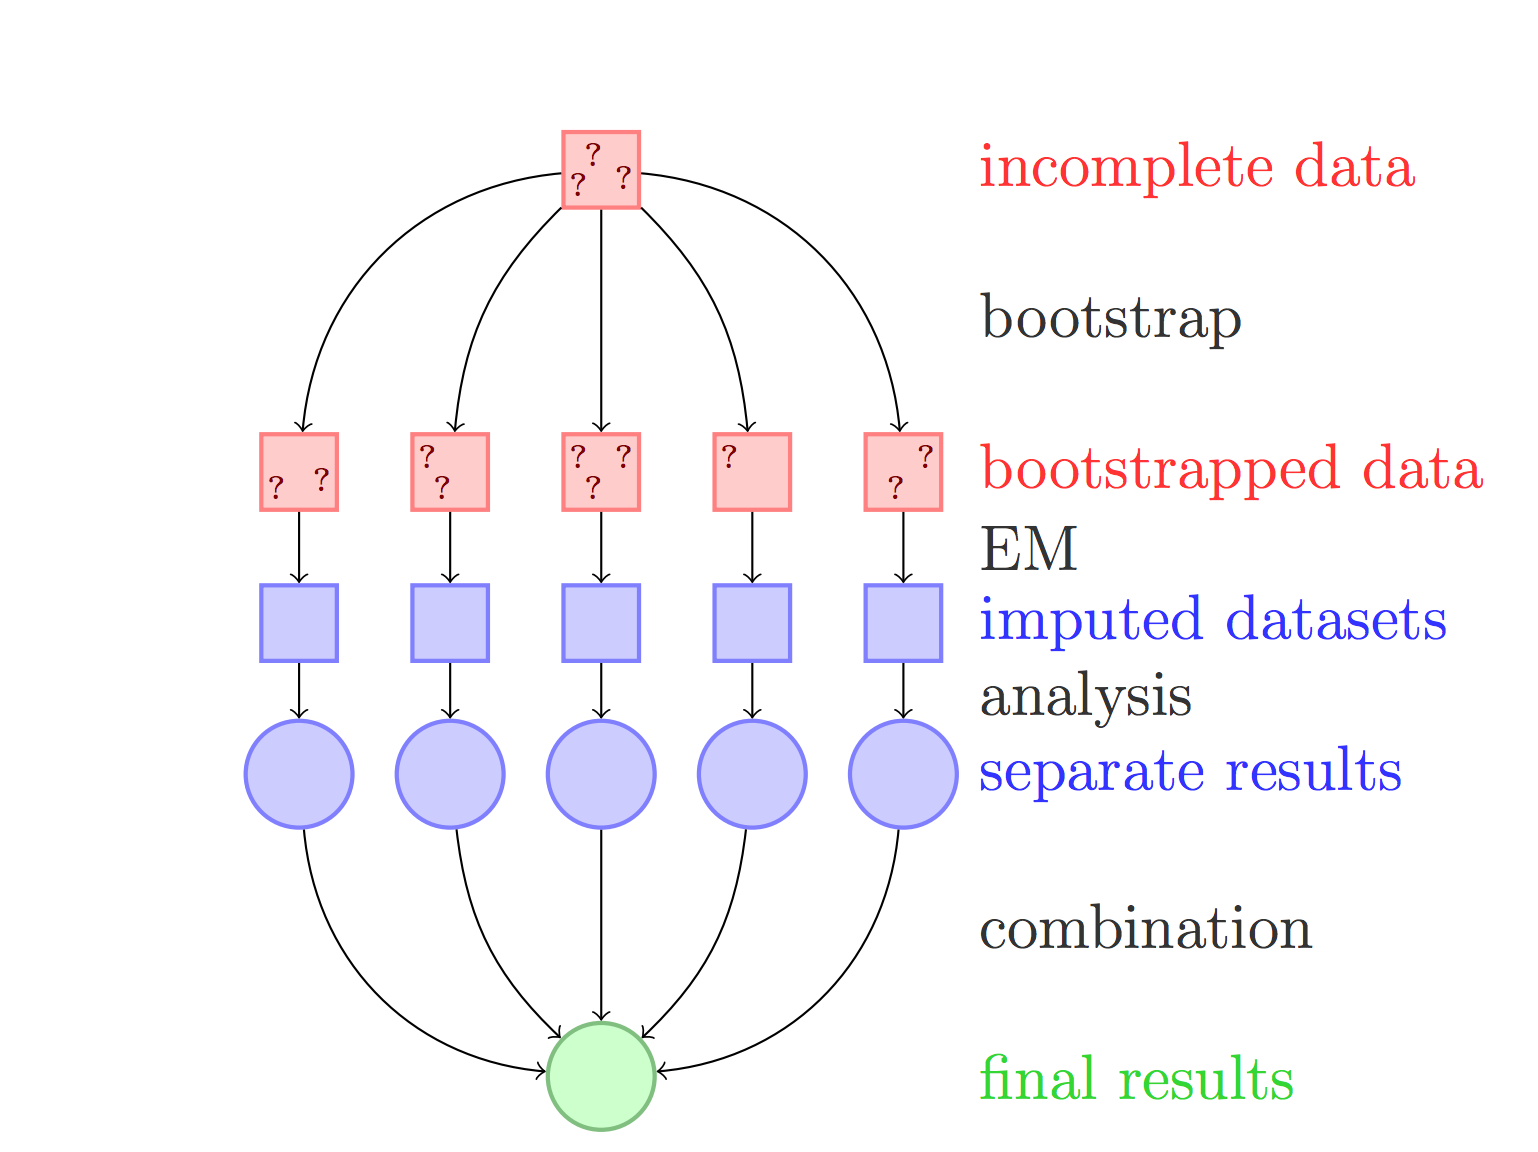
\includegraphics[width = 0.85\textwidth]{mult_imp}
\vspace{2em}\\
\tiny{Image credit: https://cran.r-project.org/web/packages/Amelia/vignettes/amelia.pdf}
}





\frame{
\frametitle{Matrix Factorization: Generalized Low Rank Models}
\begin{itemize} \small
\item<2-> Low Rank and Low Norm approaches.
\item<3-> Srebro (2004), Udell et al (2014).
\item<4-> Approximate matrix $D$ ( dimension $n \times p$) by $X'Y$. 
\item<5-> minimize \color{magenta}$ \sum_{i,j} L_{i,j} (x_i y_j, d_{ij}) + \gamma \sum \limits_{i=1}^{n} r_i(x_i) + \gamma \sum \limits_{j=1}^{p} r_j(y_j)   $.
\begin{itemize}
\item<6-> {\color{blue}$L$}: Loss function (over columns) -- quadratic, ordinal hinge, logistic, classification error etc.
\item<7-> {\color{blue}$r(.)$ }: regularization functions -- trace norm, max norm etc.
\item<8-> {\color{blue}$X$, $Y$ }: SVD good initialization.
\item<9-> {\color{blue}$k$, $\gamma$}: chosen via crossvalidation.
\end{itemize}

\item<10-> \color{magenta} Low Norm Models: \color{black} $r(x) $.
\item<11-> \color{magenta} Low Rank Models: \color{black} $Rank(X'Y) \leq k$.  
\item<12-> \color{magenta} Low Rank, Low Norm Models: \color{black} Both

\item<13-> Julia Implementation: LowRankModels 
\end{itemize}
}



\frame{
\frametitle{Interpretations: Generalized Low rank Models}

\begin{itemize}
\item<2-> Low dimensional embedding
\item<3-> Latent Variables
\item<4-> Compression
\item<5-> Denoising
\item<6-> Probabilistic Interpretation
\end{itemize}

}



\frame{
\frametitle{Interpretations: Generalized Low rank Models}

\begin{itemize}
\item<1-> Low dimensional embedding
\item<1-> Latent Variables
\item<1-> Compression
\item<1-> Denoising
\item<1-> \color{red}{\textbf{Probabilistic Interpretation} $\mathbf{\Leftarrow}$} \color{black} Equivalent to Multiple Imputation assumption when full rank. 
\end{itemize}


}









\frame{
\frametitle{Empirical Applications}

\begin{itemize}
\item<1-> \color{magenta} General Social Survey Data (GSS)

\begin{itemize}\small
\item<2->  Sociological survey: adults in randomly selected US households.
\item<3->  Data on attitudes and demographic characteristics.
\end{itemize}


\item<1-> \color{magenta} National Longitudnal Survey of Youth (NLSY)


\begin{itemize}\small
\item<4->  Longitudnal dataset: Tracking cohort of young men and women over time.
\item<5->  Data on range of economic, psychological, demographic characteristics.
\end{itemize}


\item<1-> \color{magenta}Evaluation Strategy


\begin{itemize}
\item<6-> Subsets of the data used
\item<7-> $10 \%$ observed data held-out at random.
\item<8-> Imputation models: \color{blue} Low Rank (Scaled), Low Rank (Unscaled), Trace Norm (Full Rank), Trace Norm (Low Rank), MICE
\item<9-> Loss calculated over hold out sample 
\end{itemize}

\item<1->  \color{magenta} Caveats

\end{itemize}
}

\frame{
\frametitle{Key Results: GSS}
\begin{itemize} \small
\item<2-> \small Overall Trace (Full Rank) had lowest loss, all Low Rank and Low Norm models outperformed MICE
\item<3-> \small Column-wise: $\approx  80\%$ columns had lower loss compared to MICE


\item<4-> \color{magenta} \centering \small{Summary Table}
 \color{black}
% Wed Sep  9 16:27:42 2015
\begin{table}[H] \tiny
\centering
\begin{tabular}{|c|c|c|c|c|c|} 
  \hline
 & LowRank (S) & LowRank (NS) & Trace (FR) & Trace (LR) & MICE \\ 
  \hline
Loss/($10^3$) & 18.50 & 15.80 & 14.40 & 15.80 & 20.60 \\ 
  \%age reduction over MICE& 10.10   \%& 23.40  \% & 30.10  \% & 23.00  \% & -- \\ 
  \%age cols w/ lower loss & 73.50   \% & 84.60   \% & 87.20   \% & 84.60  \% & -- \\ 
   \hline
\end{tabular}
\end{table}
\item<5-> 
\begin{center} \color{magenta}  \small{Method with  lowest loss across columns  } \end{center}
\begin{center}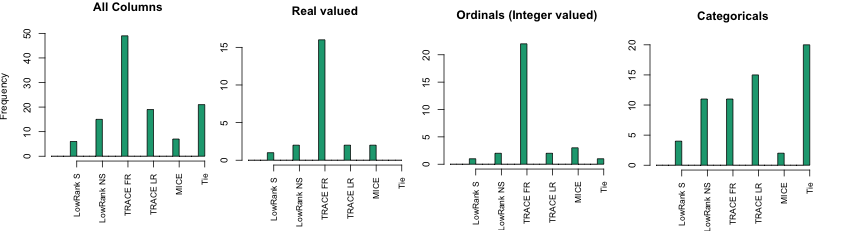
\includegraphics[width = 1.05\textwidth]{select_gss} \end{center}

\end{itemize} 
}

\frame{
\frametitle{Key Results: NLSY}
\begin{itemize} \small
\item<2-> \small Overall Trace (Full Rank) had lowest loss, all Low Rank and Low Norm models outperformed MICE
\item<3-> \small Column-wise:  $\approx  90 \%$ columns had lower loss compared to MICE


\item<4-> \color{magenta} \centering \small{Summary Table}
 \color{black}
% Wed Sep  9 16:27:42 2015
\begin{table}[H] \tiny
\centering
\begin{tabular}{|c|c|c|c|c|c|} 
  \hline
 & LowRank (S) & LowRank (NS) & Trace (FR) & Trace (LR) & MICE \\ 
  \hline
Loss/($10^3$) & 31.40 & 28.20 & 25.90 & 28.20 & 37.00 \\ 
  \%age reduction over MICE & 15.20  \% & 23.70  \%& 30.00 \%& 23.70 \% & -- \\ 
  \%age cols w/ lower loss & 75.70\% & 92.90 \%& 94.30 \% & 94.30 \%& -- \\ 
\hline
\end{tabular}
\end{table}




\item<5-> 
\begin{center} \color{magenta}  \small{Method with  lowest loss across columns}\end{center}
\begin{center}
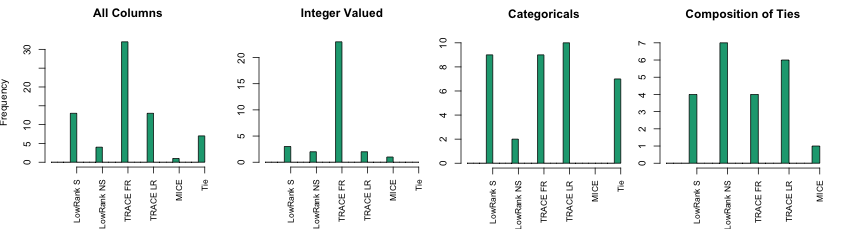
\includegraphics[width = 1.05\textwidth]{select_nlsy} \end{center}



\end{itemize} 
}








\frame{ 
\frametitle{Next Steps}

\begin{itemize}
\item<1-> Probabilistic losses
\item<2-> Max Norm regularizer 
\item<3-> Replicating missingness patterns
\item<4-> Wrapper for Multiple Imputation 
\item<5-> Extending GLRM to longitudnal data using Tensor Decomposition
\end{itemize}

}



\frame{ 
\frametitle{Next Steps}

\begin{itemize}
\item<1-> Probabilistic losses
\item<1-> Max Norm regularizer 
\item<1-> Replicating missingness patterns
\item<1-> Wrapper for Multiple Imputation 
\item<1-> {\color{red}\textbf{Extending GLRM to longitudnal data using Tensor Decomposition} $\mathbf{\Leftarrow}$ } {\color{black} Future Work.}
\end{itemize}

}






\frame{
\begin{block}{}
\color{magenta}Thank you!
\\(Comments and Suggestions Welcome)
\end{block}}

\end{document}




\frame{
\frametitle{Application 2: Simulated Dataset}

}

\frame{
\frametitle{Results}


}


\frame{
\frametitle{Results}


}